\section{Amdahl law}

In analyzing the performance of parallel computing, we consider two types of program segments: serial segments (which cannot be parallelized) and parallelizable segments. 
The total execution time depends on the proportion of each.
\begin{figure}[H]
    \centering
    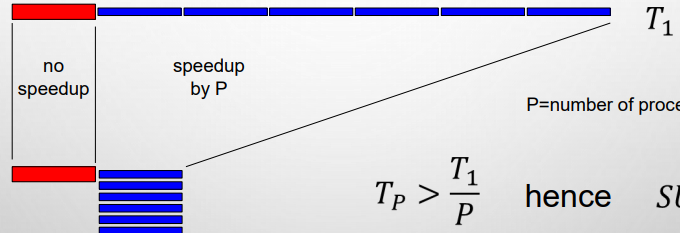
\includegraphics[width=0.75\linewidth]{images/am.png}
    \caption{Amdahl model}
\end{figure}
As depicted in the Amdahl model, when using more than one processor, the speedup ($\text{SU}_P$) is always less than the number of processors ($P$). 
The relationship can be expressed as:
\[T_P>\dfrac{T_1}{P}\implies \text{SU}_P<P\]
Here, $T_P$ is the time taken with $P$ processors, and $T_1$ is the time for a serial execution.

In a program, the parallelizable portion is often represented by a fixed fraction, $f$. 
\begin{figure}[H]
    \centering
    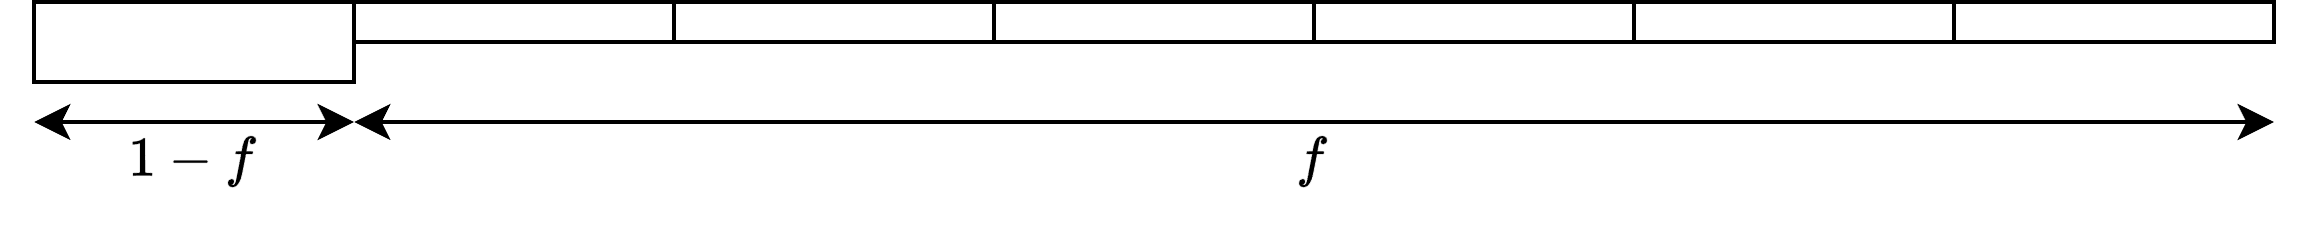
\includegraphics[width=0.75\linewidth]{images/am1.png}
    \caption{Serial model}
\end{figure}
Using the serial version of the model, the speedup function $\text{SU}(P, f)$ is derived as follows:
\[\text{SU}(P,f)=\dfrac{T_1}{T_P}=\dfrac{T_1}{T_1(1-f)+\frac{T_1f}{P}}=\dfrac{1}{1-f+\frac{f}{P}}\]
As the number of processors $P$ approaches infinity, the speedup is limited by the serial portion:
\[\lim_{P\rightarrow\infty}\text{SU}(P,f)=\dfrac{1}{1-f}\]
This shows that even with an infinite number of processors, the maximum speedup is constrained by the serial fraction of the program. 
For example, if 90\% of the program is parallelizable ($f > 0.9$), there is little benefit to using more than 10 processors.

\subsection{Gustafson law}
In contrast to Amdahl's Law, John L. Gustafson proposed a different view in 1988, challenging the assumption that the parallelizable portion of a program remains fixed. 
Key differences include:
\begin{itemize}
    \item The parallelizable portion of the program is not a fixed fraction.
    \item Absolute serial time is fixed, while the problem size grows to exploit more processors.
    \item Amdahl's law is based on a fixed-size model, while Gustafson's law operates on a fixed-time model, where the problem grows with increased processing power.
\end{itemize}
The speedup in Gustafson's model is expressed as:
\[\text{SU}(P)=\dfrac{T_1}{T_P}=\dfrac{s+P(1-s)}{s+1-s}=s+P(1-s)\]
Here, $s$ is the fixed serial portion of the program.
As a result, this model suggests linear speedup is possible as the number of processors increases, especially for highly parallelizable tasks. 
Gustafson's law is empirically applicable to large-scale parallel algorithms, where increasing computational power enables solving larger and more complex problems within the same time frame.

\subsection{Summary}
Amdahl's Law assumes that the overall computing workload remains constant, and thus adding more processors merely reduces execution time for the same task. 
This makes Amdahl's model practical for scenarios where the problem size is fixed, but speedup is limited by the non-parallelizable (serial) portion of the task.

On the other hand, Gustafson's Law takes a more expansive view, arguing that as computing power increases, the problem size grows accordingly. 
More processors allow for deeper, more detailed analysis, which wouldn't have been feasible with limited computational resources.
Increasing the power of computation enables more comprehensive simulations, something impossible within fixed-size, limited-time models.

In essence, Amdahl's law focuses on reducing time for fixed workloads, while Gustafson's law encourages scaling workloads to take full advantage of increased processing power.